\documentclass[aspectratio=169]{beamer}

\usepackage{fontspec}
\usepackage[croatian]{babel}
\usepackage{graphicx}
\usepackage{booktabs}
\usepackage{tikz}

\usetheme{Madrid}
\usecolortheme{default}

\definecolor{smrblue}{HTML}{1F4E79}
\definecolor{smrorange}{HTML}{C65D28}
\definecolor{smrgray}{HTML}{F3F5F7}

\setbeamercolor{palette primary}{bg=smrblue,fg=white}
\setbeamercolor{palette secondary}{bg=smrblue,fg=white}
\setbeamercolor{palette tertiary}{bg=smrorange,fg=white}
\setbeamercolor{frametitle}{bg=smrblue,fg=white}
\setbeamercolor{title}{fg=white,bg=smrblue}
\setbeamercolor{block title}{bg=smrblue,fg=white}
\setbeamercolor{block body}{bg=smrgray,fg=black}
\setbeamertemplate{navigation symbols}{}
\setbeamertemplate{footline}[frame number]

\graphicspath{{figures/}}

\title{Analiza javnog mnijenja o sigurnosti SMR tehnologije i prihvatljivosti izgradnje u blizini mjesta stanovanja}
\author{Tim E}
\date{}

\newcommand{\imageplaceholder}[2]{%
  \begin{tikzpicture}
    \node[draw=smrblue, rounded corners, fill=smrgray, minimum width=#1, minimum height=#2, align=center] {
      \textbf{Rezervirano mjesto za sliku}\\[0.35em]
      Slobodna slika uz atribuciju\\
      npr. SMR, nuklearna elektrana ili elektroenergetska mreža
    };
  \end{tikzpicture}%
}

\begin{document}

\begin{frame}[plain]
  \begin{tikzpicture}[remember picture,overlay]
    \fill[smrblue] (current page.south west) rectangle (current page.north east);
    \fill[smrorange] (current page.south west) rectangle ([xshift=0.18\paperwidth]current page.north west);
  \end{tikzpicture}
  \vspace{1.3cm}
  {\color{white}\Huge\textbf{Analiza javnog mnijenja o SMR tehnologiji}}\\[0.5cm]
  {\color{white}\Large Sigurnost, prihvatljivost i državne subvencije}\\[1.2cm]
  {\color{white}\large Tim E}
\end{frame}

\begin{frame}{Istraživački fokus}
  \begin{columns}[T]
    \begin{column}{0.58\textwidth}
      \begin{block}{Analizirana pitanja}
        \begin{itemize}
          \item \textbf{P9}: najveća percipirana prednost SMR tehnologije
          \item \textbf{P10}: opravdanost državnog subvencioniranja razvoja SMR tehnologije
        \end{itemize}
      \end{block}
      \vspace{0.4cm}
      \begin{block}{Kontekst}
        Rezultati se tumače u širem okviru percepcije sigurnosti, koristi i prihvatljivosti SMR tehnologije.
      \end{block}
    \end{column}
    \begin{column}{0.38\textwidth}
      \imageplaceholder{4.2cm}{4.5cm}
    \end{column}
  \end{columns}
\end{frame}

\begin{frame}{Podaci i metoda}
  \begin{columns}[T]
    \begin{column}{0.52\textwidth}
      \begin{itemize}
        \item Izvor: \texttt{anketa\_utorak.xlsx}
        \item Analizirana su pitanja P9 i P10
        \item Usporedbe prema spolu, dobi, obrazovanju, zaposlenosti i županiji
      \end{itemize}
    \end{column}
    \begin{column}{0.44\textwidth}
      \begin{block}{Statistička obrada}
        \begin{itemize}
          \item frekvencije i postotci
          \item križne tablice
          \item hi-kvadrat testovi
          \item Cramérov \(V\)
        \end{itemize}
      \end{block}
    \end{column}
  \end{columns}
\end{frame}

\begin{frame}{P9: percipirana prednost SMR tehnologije}
  \centering
  
\includegraphics[width=0.88\textwidth]{p9_odgovori.pdf}
\end{frame}

\begin{frame}{P10: stav prema državnim subvencijama}
  \centering
  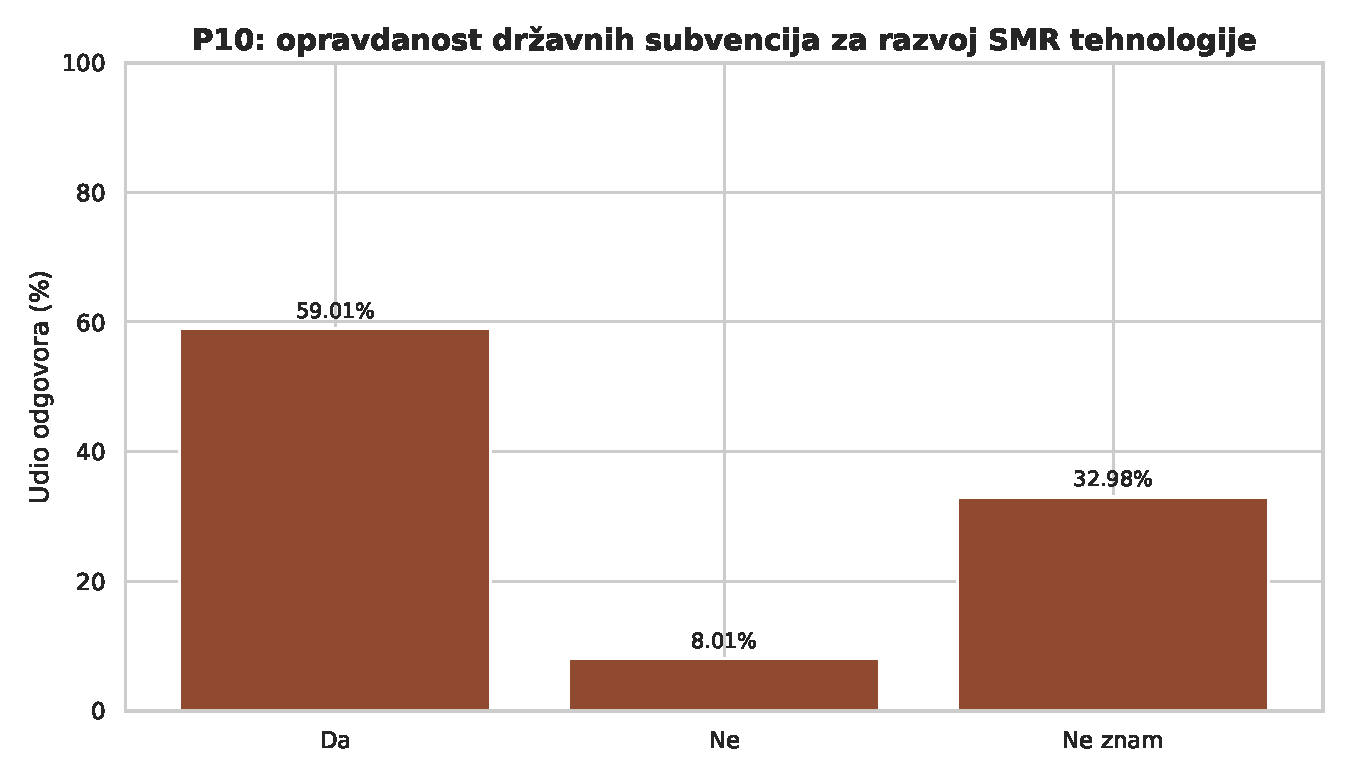
\includegraphics[width=0.88\textwidth]{p10_odgovori.pdf}
\end{frame}

\begin{frame}{Demografske razlike}
  \begin{block}{Statistički značajne povezanosti}
    Nakon spajanja kategorija s manje od pet opažanja, značajne su povezanosti \textbf{Spol--P9} i \textbf{Obrazovanje--P10}.
  \end{block}
  \vspace{0.3cm}
  \begin{columns}
    \begin{column}{0.49\textwidth}
      \centering
      
\includegraphics[width=\textwidth]{povezanost_spol_p9_kratko.pdf}
    \end{column}
    \begin{column}{0.49\textwidth}
      \centering
      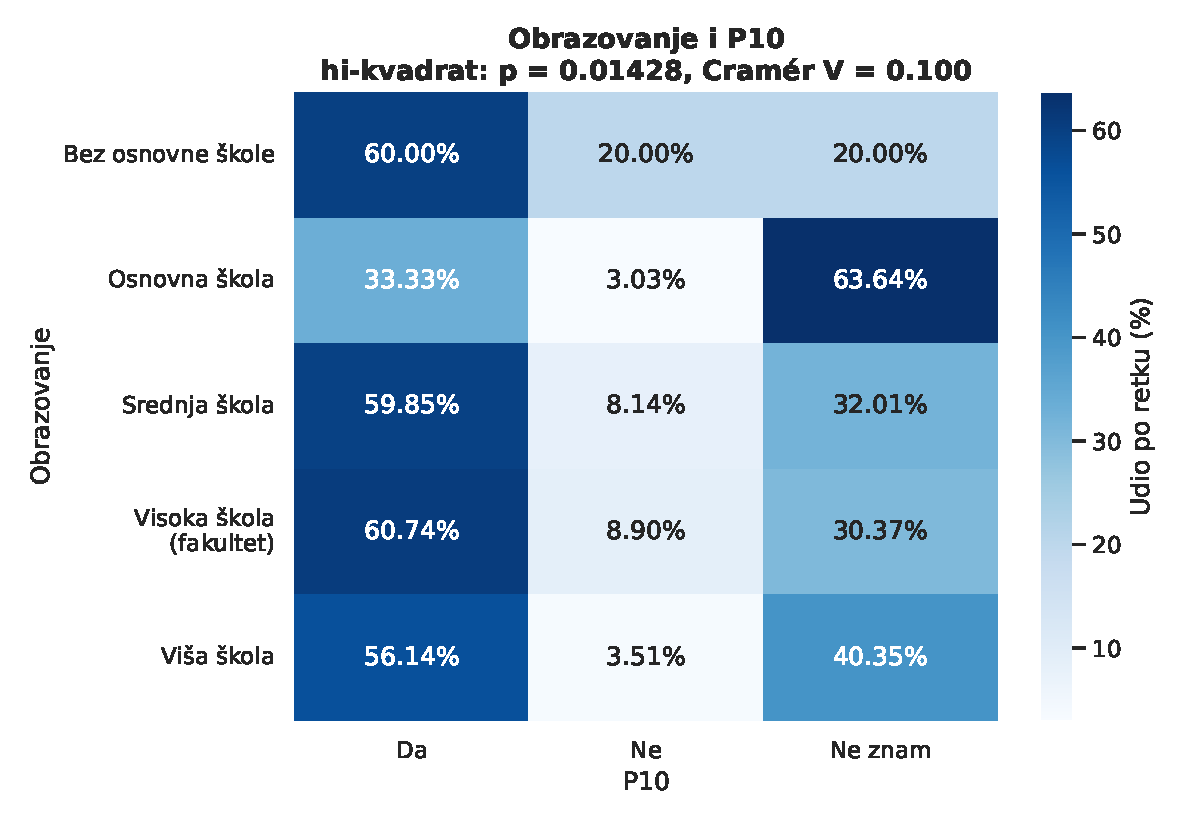
\includegraphics[width=\textwidth]{povezanost_obrazovanje_p10_kratko.pdf}
    \end{column}
  \end{columns}
\end{frame}

\begin{frame}{Povezanost P9 i P10}
  \begin{block}{Interpretacijsko pitanje}
    Jesu li ispitanici koji ističu određenu prednost SMR tehnologije skloniji podržati državne subvencije?
  \end{block}
  \vspace{0.4cm}
  \begin{itemize}
    \item U izvještaju se koristi križna tablica P9 \(\times\) P10.
    \item Zaključak o povezanosti temelji se na hi-kvadrat testu i Cramérovu \(V\).
  \end{itemize}
\end{frame}

\begin{frame}{P9 i P10: grafički prikaz povezanosti}
  \centering
  
\includegraphics[width=0.83\textwidth]{povezanost_p9_kratko_p10_kratko.pdf}
\end{frame}

\begin{frame}{Zaključak}
  \begin{columns}[T]
    \begin{column}{0.56\textwidth}
      \begin{block}{Ključne poruke}
        \begin{itemize}
          \item Dopuniti dominantnim odgovorom na P9.
          \item Dopuniti dominantnim odgovorom na P10.
          \item Dopuniti najvažnijim statističkim nalazom.
        \end{itemize}
      \end{block}
    \end{column}
    \begin{column}{0.38\textwidth}
      \imageplaceholder{4.2cm}{4.5cm}
    \end{column}
  \end{columns}
\end{frame}

\end{document}
